\documentclass[11pt, a4paper]{article}
\usepackage[spanish]{babel}
\usepackage[utf8]{inputenc}
\usepackage{mathpazo}
\usepackage{geometry}
\geometry{a4paper,
  left=1.2in,
  right=1.2in,
  top=1.2in,
  bottom=1.2in
}
\usepackage{titlesec}
\usepackage{fancyhdr}
\usepackage{setspace}
\usepackage{graphicx}
\usepackage{float}
\usepackage{microtype}
\usepackage{amsmath, amssymb, amsthm}

\pagestyle{fancy}
\fancyhf{}
\renewcommand{\headrulewidth}{0.8pt}
\fancyfoot[C]{\thepage}
\fancyhead[L]{\nouppercase{\rightmark}}
\fancyhead[R]{\nouppercase{Proyecto de LaTeX}}

\onehalfspacing

\setlength{\parskip}{1.8em}

\newcommand{\ensayoTitulo}[2]{%
  \begin{center}
    \vspace*{1cm}
    {\fontsize{36}{38}\selectfont\textbf{#1}} \\
    \vspace{0.4cm}
    {\fontsize{18}{20}\selectfont\textit{#2}}
    \vspace*{1.5cm}
    \hrule
    \vspace*{0.3cm}
  \end{center}
}

\begin{document}

\ensayoTitulo{El cuantificador universal}

Pocas disciplinas exigen tanta formalidad y precisión como la lógica. Aunque también requiere ser realizada de la manera más eficaz y óptima posible. Es ese balance entre rigor y eficiencia el que dota a la lógica de su elegancia característica . Y es por esto que, para su adecuada práctica,  requerimos de las herramientas necesarias para cumplir con sus estándares. 

En esta disciplina se trabaja con operadores lógicos (negación, conjunción, disyunción, implicación, etc.), variables y  predicados. En su estudio, se analiza qué proposiciones se cumplen para qué clase de variables. Y es evidente que se requiere de alguna forma, indicar para cuántas  variables se cumple alguna proposición. De esta forma, surge la necesidad de un \emph{cuantificador}. 

Naturalmente, los lógicos de la época no demoraron en idear sus propios símbolos para representar que un predicado se cumple (o no), para alguna, o para todas las variables. 
Uno de los pioneros en esto fue Gottlob Frege, quien utilizó los cuantificadores por primera vez en 1879 en su obra “Begriffsschrift”.  Su notación no era la más intuitiva, ni la más agradable estéticamente (Fig. 1.1); se asemejaba más a diagramas de circuitos electrónicos que a los símbolos simplificados que usamos hoy en día. Es por esto que a pesar de ser fundacional, la notación de Frege no se utiliza hoy en día. 

\begin{figure}[H]
    \centering
    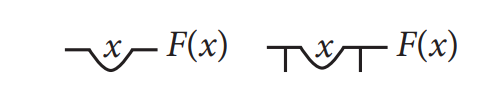
\includegraphics[width=0.7\textwidth]{cuantificador_frege.png}
    \caption{El cuantificador universal de Gottlob Frege (Rojas González, 2018, p. 166). Imagen recuperada del libro.}
    \label{fig:frege}
\end{figure}

Otro ejemplo de notación que precede a la que conocemos actualmente surgió en 1885, gracias a Charles Sanders Peirce. Él utilizó las letras griegas $\varPi$ y $\varSigma$ para el cuantificador universal y existencial respectivamente, colocándoles las variables como subíndice. 

\begin{center}
$\varPi_x$ , $\varSigma_x$
\end{center}

La notación de Peirce fue bastante influyente y se utilizó por muchos años, tantos como para que Kurt Gödel la utilizara en algunos de sus trabajos. Sin embargo, en 1933 aparecería por primera vez el cuantificador universal tal y como lo conocemos hoy en día. 

En el año ya mencionado, el alemán Gerhard Gentzen defiende su tésis doctoral en la universidad de Gotinga, donde utiliza una letra A mayúscula volteada de cabeza para representar al “para todo”. Pero, \emph{¿por qué?}

En su tésis, el mismo Gentzen admite haberse inspirado en Giuseppe Peano, el responsable de idear el cuantificador existencial que usamos en la actualidad. En 1897 Peano tomó la letra E mayúscula y la reflejó horizontalmente, creando así el icónico símbolo $\exists$  de “existe”. Para crear el $\forall$, simplemente imitó la técnica del italiano. De cierto modo parecía admirarlo, ya que fue el mismo Gentzen quien probó la consistencia de los axiomas de la aritmética de Peano unos años después. 

En cuanto a la elección de la letra, Gerhard Gentzen escogió la “A” para representar el “para todo” por una razón muy simple; la palabra \emph{“alle”} en alemán se traduce a “todos”, entonces la letra inicial de esta palabra es el motivo. 

El cuantificador universal nació en una época de imperialismo y de extrema tensión entre naciones,  y la vida de su creador lo refleja a la perfección. 
Se dice que Gentzen fue un matemático genial, lo suficientemente genial como para llegar a ser asistente del mismísimo David Hilbert en la universidad de Gotinga. Pese a ser indudablemente brillante, carecía de convicciones, y llegó a tomar medidas moralmente cuestionables para su beneficio personal. 

A pesar de no tener interés alguno en la política, se afilió al Partido Nacional Socialista Alemán de los Trabajadores, y se unió a la asociación nazi de profesores, todo con la finalidad de asegurar una ocupación académica o de docente de matemáticas. 

\begin{figure}[H]
    \centering
    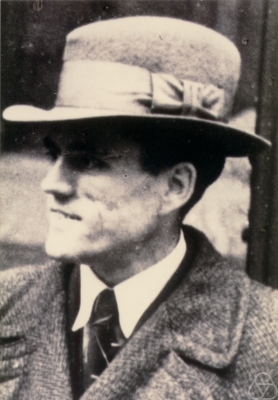
\includegraphics[width=0.7\textwidth]
    {Gerhard_Gentzen.jpg}
    \caption{Gerhard Gentzen en Praga, 1945.}
    \label{fig:gentzen}
\end{figure}
 % HOLAAAA!!! AQUI NO SUPE PONER BIEN LA REFERENCIA EN EL \CAPTION PERO DEBERÍA DECIR ESTO:
 %(Figura 1.2) Gerhard Gentzen en Praga, 1945. Por Eckart Menzler-Trott - https://opc.mfo.de/detail?photo_id=8540, CC BY-SA 2.0 de, https://commons.wikimedia.org/w/index.php?curid=7238093
 
% Y TAMBIÉN SI SABES HACER LA FOTO MAS PEQUEÑA ESTARÍA EXCELENTE 

Al final, las consecuencias de sus acciones alcanzaron a Gentzen; Llámese destino, o karma.  Cuando Praga fue liberada, Gentzen fue arrestado y murió de desnutrición en agosto de 1945. 
Sin embargo, su trabajo fue altamente influyente en los avances lógicos de la época, y su creación, sin lugar a dudas, vivirá por generaciones. 

\end{document}